\subsection{The Model}\label{sec:themodel}
This section will showcase the model made to express the design from \myref{cha:Design}.
For simplicity the the model in this chapter has been split into two parts, an initializing phase and the main loop.
Before the template is shown the code for the system will be presented.
The template has local code which can be seen on \myref{device_local}.
This code contains functions which encapsulate many updates from the template, which would otherwise clutter the template with too many specifics.

The global code for the system can be seen on \myref{uppaal_Global}.
This is where the system sends information from one device to another, when one device transmit it will change the global values, while the receiving devices will get the global values and put them locally.
Another important thing to note is the broadcast channel transmit, which will be used as descibred in \myref{UPPAAL_Models}.

\noindent\begin{minipage}{0.47\textwidth}
\begin{lstlisting}[style=UPPAAL,
caption={Local code for Device.}, label={device_local}]
// Place local declarations here.
clock x;
clock transmit_time;
int k = -1;                     //Timeslot
bool Connected = false;

// Local copies of globals
// Number of devices connected
int local_n = 0; 
// Current time slot in the frame
int local_i = 0;

void increment_Slot(){
    local_i = (local_i % local_n)+1;
}

void receive()
{
    local_i = i;
    local_n = n;
}

void join_Network(){
    k=n;
    n = n+1;
    local_n = local_n+1;
    Connected = true;
    Connected_Counter++;
}

void create_Network(){
    i = 0;
    n = 2;
    k = 1;
    local_i = 0;
    local_n = 2;
    Connected_Counter = 1;
    Connected = true;
    x:=0;
}

void make_Payload(){
    i = local_i;
    n = local_n;
}

\end{lstlisting}
\end{minipage}\hfill
\begin{minipage}{0.47\textwidth}
\begin{lstlisting}[style=UPPAAL,
caption={Code for the global declarations.}, label={uppaal_Global}]
// Place global declarations here.
// Number of Timeslots connected
int n = 0;         
// Current time slot in the frame
int i = 0;            
//Global Counter for Connected Devices                    
int Connected_Counter = 0;
//Timeslot Length
const int Delta = 250;                 
const int Delta_Proc = Delta/5;
const int Real_Tx_Time = Delta/2;
const int Tx_Time = Delta_Proc + Real_Tx_Time;
const int Initial_Wait_Time = Delta*3;
const int Startup_Time = Initial_Wait_Time*2;
clock time;

//Channel
broadcast chan transmit;

//Device Creation
const int N = 4;
typedef int[1,N] id_t;
\end{lstlisting}
\end{minipage}

Finally to instantiate the system, a system declaration is needed which can be seen on \myref{UPPAAL_System_Dcl}.
This creates $N$ devices each with a unique ID from $1 - N$ because of the code seen on \myref{uppaal_Global}, at the comment Device Creation.

\begin{lstlisting}[style=UPPAAL,
caption={Code for system declarations.}, label={UPPAAL_System_Dcl}]
system Device;
\end{lstlisting}

\begin{figure}
  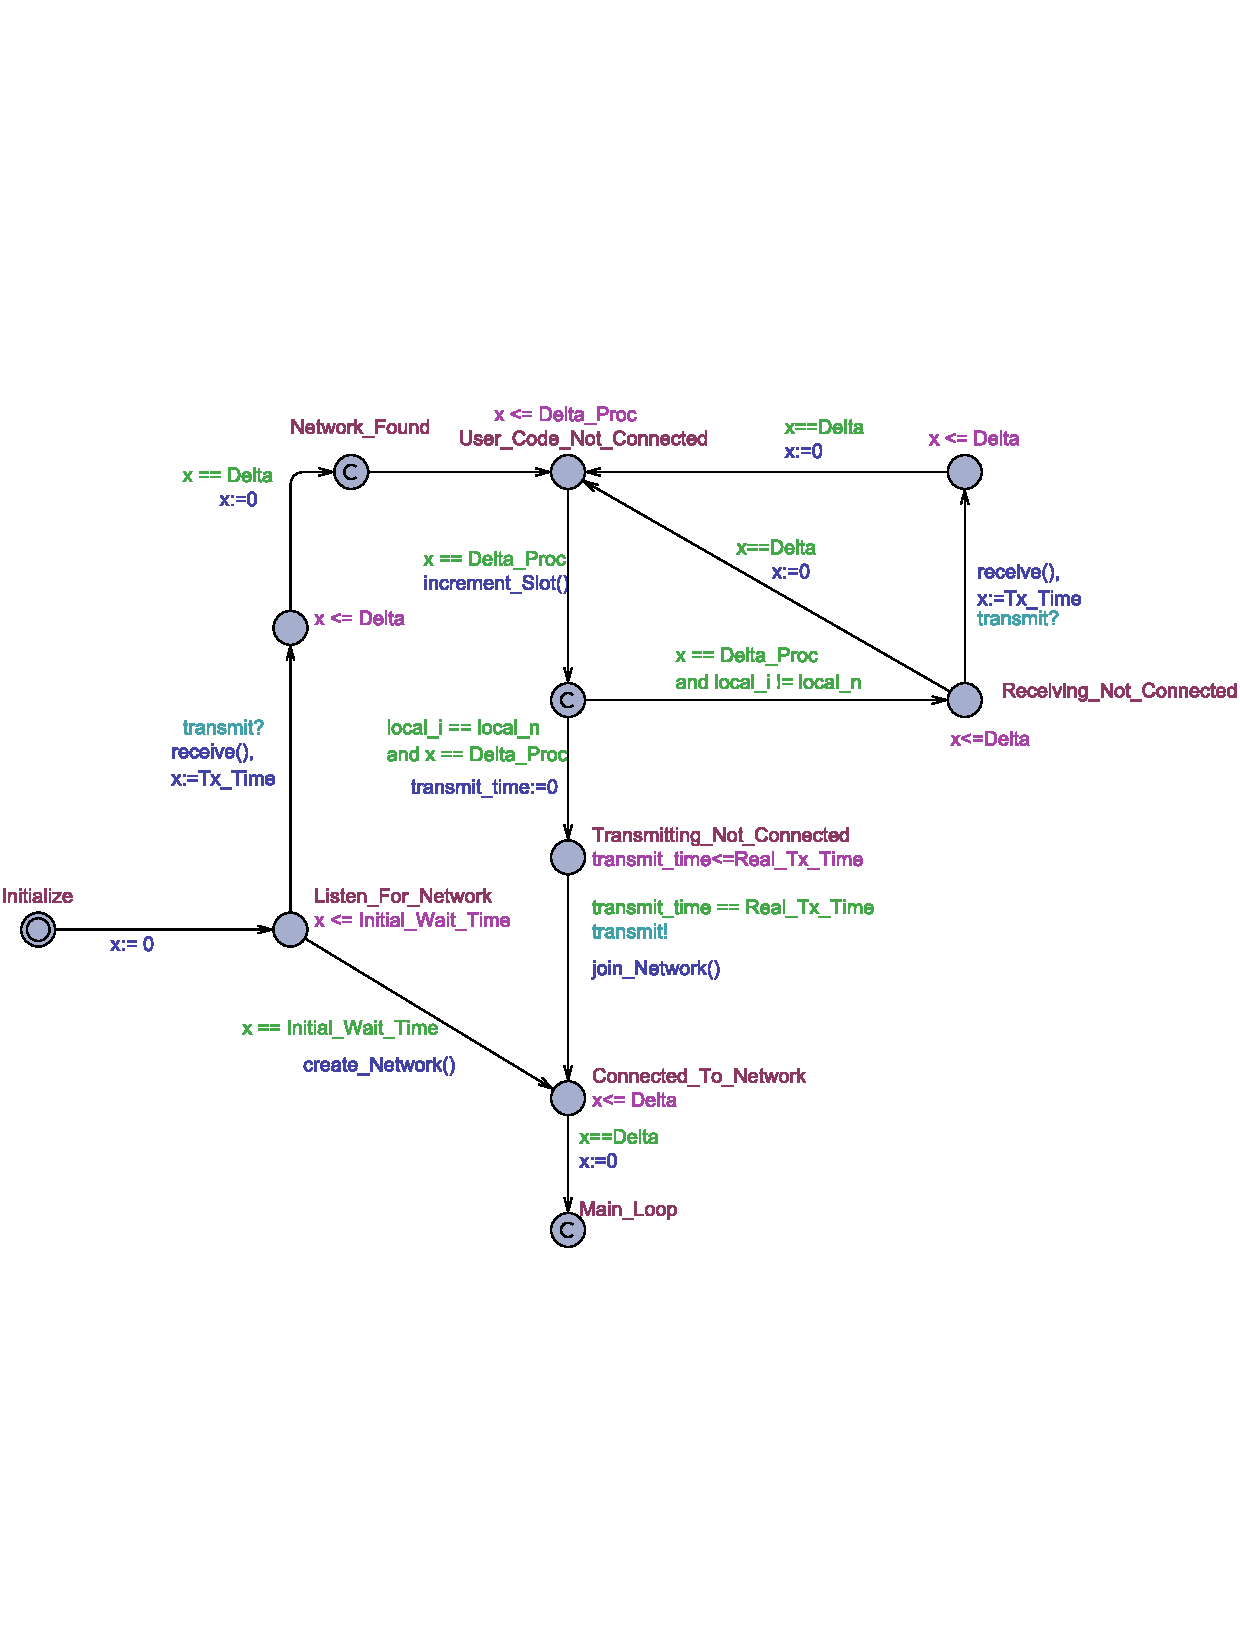
\includegraphics[width=1\textwidth]{Figures/Model/Device_Connecting_MultiStart.pdf} 
\caption{UPPAAL Model showing how the devices initialize.}
\label{fig:UPPAAL_Intitialization}
\end{figure}

\bigskip \noindent

Firstly the devices will nondeterministically leave the initial stage, and start listening for a network.
When they are done listening and have not found a network, they will create a network themselves, by firing the edge towards the \texttt{Connected\_To\_Network} location.
The device will setup the initial values for the network, change its boolean \texttt{Connected} to true, this all happens in the function \texttt{create\_Network()}. 
The device will move onwards towards the main loop, which will be shown later.
When the devices listen and find the newly created network, they will fire the other edge, where the broadcast channel \texttt{transmit} is seen.
The device will stay in this location until the communication phase of the time-slot is complete, which is until \texttt{Delta}, and then it will continue towards the committed location \texttt{Network\_Found} and reset the clock \texttt{x} to zero.
This location is committed as its purpose is simply visual working as a context switch between having found a network and entering the loop to wait for the empty slot.
When it has just received a transmission, the device which just transmitted will according to \myref{cha:Design} be performing user code, and therefore the device trying to connect should be waiting for the next time-slot so the other devices are ready to receive again.

\bigskip \noindent
When \texttt{x} is equal to \texttt{Delta\_Proc}, the time designated to perform user code, the device will fire the edge to the committed location directly under \texttt{User\_Code\_Not\_Connected} once again.
In this location when \texttt{x} is not zero, the device checks whether \texttt{i}, the current time-slot, is the empty-time slot, if it is the device will transmit and ultimately connect to the network increasing the number of time-slots in the network according to the specifications in \myref{cha:Design}.
If the empty slot was not the current time-slot, the device will instead go to the location \texttt{Receiving\_Not\_Connected} where it will receive the other devices' transmissions, once again reset \texttt{x} to zero and loop until eventually the empty slot occurs, where it will connect to the network.
The model can be seen on \myref{fig:UPPAAL_Connected}.

\begin{figure}
  
\includegraphics[width=1\textwidth]{Figures/Model/Device_Connected.pdf} 
\caption{UPPAAL Model showing the devices' main loop.}
\label{fig:UPPAAL_Connected}
\end{figure}

When a device has been connected to a network it will instantly move to the location main loop, where it will perform the actions as described in the pseudocode of \myref{cha:Design}.

First it moves to a location \texttt{User\_Code} where it will perform user code until the the clock \texttt{x} is equal to \texttt{Delta\_Proc}.
As soon as this is the case the device will move on to a committed location where it will choose to either transmit or receive depending on whether or not the current time-slot belongs to the device or not.
When a device has transmitted a transmission, it will move to a waiting location where it will wait until the time-slot has officially ended, which is when the clock \texttt{x} is equal to \texttt{Delta}, reset the clock \texttt{x} and then it will execute the main loop once again.
This also happens when the device in the empty slot is transmitting, the device waits before starting the main loop.
When the device is in the location \texttt{Receiving}, if nothing has been transmitted and the clock \texttt{x} is equal to \texttt{Delta} the device will go increment its \texttt{i\_local} value reset the clock \texttt{x} and restart the main loop. 
This case happens whenever the empty slot is the current time-slot and no new device is trying to connect to the network.
According to the specification of \myref{cha:Design} devices which receive a transmission will synchronize to the clock of the transmitting device, this is implemented in the system as the update \texttt{x:=Tx\_Time}, where \texttt{Tx\_Time} is the sum of \texttt{Delta\_Proc} and \texttt{Real\_Tx\_Time}, so it is the time the transmitting device has spent until it is done transmitting.
A function to calculate this synchronized time will be require to implement the model on an Arduino.

\subsection{Verifying the Model}\label{sec:verifyingTheModel}

As mentioned in \myref{subsec:uppaal} it is possible to make queries to verify that some given properties are true.
\myref{sec:Pseudo} contains statements which should be true for a correctly connected network.
These statements can be written as queries in UPPAAL, which the tool will then determine to be correct or not. 
The queries described here will be tested with a system consisting of up to 6 devices, it is recommended to not go much higher than 6 in one system as the queries computation time increase dramatically.
The queries for the system will be given one by one with along with a description of what they represent.

The computer used for all the tests is a laptop with an Intel i3 processor with a clock speed of 2.3 GHz, and 4 GB ram, running Windows 8.

\noindent\begin{minipage}{\textwidth}
\begin{lstlisting}[style=UPPAAL, title={This query requires that eventually if all devices are connected, then no pair of devices have the same \texttt{k}, unless the pair consists of the same two devices.}]
1. A<> forall(i : id_t) forall(j : id_t) Device(i).Connected and
         Device(j).Connected and (Device(i).k == Device(j).k imply i == j)
\end{lstlisting}
\end{minipage}

When UPPAAL runs this query on the model it will return false.
It is possible to ask UPPAAL for the trace for why the property was not true.
This feature shows that it was not true because in the case that no device ever leaves the initial state. 
Then no device will ever be connected, making the query false.
To counteract this an invariant has been added to the model as shown on \myref{UPPAALInvariant}.

\begin{wrapfigure}[11]{r}{0.5\textwidth}
  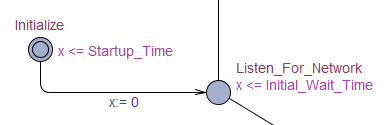
\includegraphics[width=0.5\textwidth]{Figures/Model/InvariantOnStartup.png} 
\caption{Addition of an invariant on the initial location.}
\label{UPPAALInvariant}
\end{wrapfigure}

This will make sure that when 100 time-slots has passed all of the devices will be forced to leave the initial location.
So after this change query number 1 can be checked for once again with 6 devices.
The result of the query will still yield a false result, and the trace shows that two instances of the device template has the same k value, which means they have the same time-slot, which is not supposed to happen.
When looking through the trace it shows that the devices left the initial location at roughly the same point in time which seemed to be the cause of the error.
In order to fix this, very little has to change.
A global clock \texttt{startup} will be added, and a guard on the edge leaving the initial location will require the clock being greater or equal to \texttt{Startup\_Time}, and when a device fires this edge, it will then update the clock \texttt{startup} to zero, which makes sure that a device will only leave the initial location in the interval which is \texttt{Startup\_Time}.

The change in the code will be an addition of the clock, which can be seen on \myref{lst:Clock_Addition}
\begin{lstlisting}[style=UPPAAL, caption={Addition of the \texttt{startup} clock}, label={lst:Clock_Addition}]
clock startup;
\end{lstlisting}

\begin{wrapfigure}[12]{r}{0.5\textwidth}
    \hspace{-10pt}
    \vspace{-10pt}
  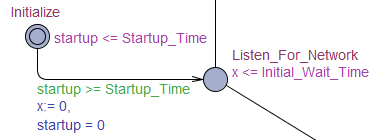
\includegraphics[width=0.5\textwidth]{Figures/Model/IntervalStartup.png} 
\caption{The additions to the model to implement that a device will leave the initial location with a minimum interval equal to \texttt{Startup\_Time}.}
\label{fig:OneStartUp}
\end{wrapfigure}

The final additions can be seen on \myref{fig:OneStartUp}.
If query number 1 is run once again with 6 devices on the tests setup, it will return true after a computation-time time of 37.7 seconds.
This means that with these changes to the model, a network will be created correctly.
However, it is a problem that multiple devices cannot be turned on at the same time, therefore this problem will be investigated further in \myref{chap:MDA-CCRC}, but for now the rest of the queries will be introduced and explained.

\begin{lstlisting}[style=UPPAAL, title={The query requires that there is no deadlock in the system, it will result in true with a computation-time of 84.8 seconds when run on the test setup with 6 devices.}]
2. A[] not deadlock
\end{lstlisting}

\begin{lstlisting}[style=UPPAAL, title={This query requires that no pair of devices are in the \enquote*{Transmitting} state at the same time. The query will, when run with 6 devices on the test setup, result in true with a computation-time of 67.7 seconds.}]
3. A[] forall(i : id_t) forall(j : id_t) 
      ((Device(i).Transmitting and Device(j).Transmitting) 
    or (Device(i).Transmitting and Device(j).Transmitting_Not_Connected) 
    or (Device(i).Transmitting_Not_Connected and Device(j).Transmitting_Not_Connected)) 
    imply i==j
\end{lstlisting}

\begin{lstlisting}[style=UPPAAL, title={This query requires that if two devices are both in the location \texttt{User\_Code} they then have the same value of their \texttt{local\_i}}. This imply that they are synchronised. When run with 6 devices the query will result in true with a computation-time of 40.7 seconds. ]
4. A[] forall(i : id_t) forall(j : id_t) Device(i).User_Code and 
        Device(j).User_Code imply Device(i).local_i == Device(j).local_i
\end{lstlisting}

\begin{lstlisting}[style=UPPAAL, title={This query requires that if a device \texttt{i} and a device \texttt{j} is both connected, they then have the same value of their \texttt{local\_n}. If they were different it would mean that they are not in the same network, and as such would have different numbers of time-slots in their networks. But the system model makes sure that this is not the case. When run with 6 devices it will return true after 86.6 seconds.}]
5. A[] forall(i : id_t) forall(j : id_t) 
    Device(i).Connected and Device(j).Connected 
    imply Device(i).local_n == Device(j).local_n
\end{lstlisting}

\begin{lstlisting}[style=UPPAAL, title={This query requires that it is always true that all devices never has the the time-slot which one of the devices has locally as the empty slot. If any device did have this, it would mean that a device was out of sync, since it did not know which time-slot would be the empty one. When run this query will when run with instances of the devices tempalte result in true after a computation-time of 66.0 seconds. }]
6. A[] forall(i : id_t) forall(j : id_t) Device(i).k != Device(j).local_n
\end{lstlisting}

\begin{lstlisting}[style=UPPAAL, title={This query requires that if a device is connected it has a \texttt{k} value between \texttt{0} and \texttt{n}, which is the number of time-slots in the frame. This query will when run with 6 devices result in true with a computation-time of 65.3 seconds.}]
7. A[] forall(i : id_t) 
    Device(i).Connected and Device(j).Connected 
    imply Device(i).k < n and Device(i).k > 0
\end{lstlisting}

\begin{lstlisting}[style=UPPAAL, title={The query requires that if a device is connected, is it then true that the number of devices connected to a network is equal to one less the number of time-slots in the frame of a network. When run with 6 devices the result of the query will be true with a computation-time of 23.8 seconds. }]
8. A[] forall(i : id_t) Device(i).Connected imply Connected_Counter == n-1
\end{lstlisting}

All of these queries will now yield a true result, after the changes shown in this section making sure there is a interval between each activation of a device, when run with 6 devices on the model presented in this chapter.
All the queries were run on the same laptop.
Note that queries have been added to verify the model beyond the ones derived from the statements in \myref{sec:Pseudo}, an example is query 2.

The queries 1, 7 and 8 together make up the statement (e) from \myref{sec:Pseudo}, since if no devices have the same time-slot k and if the number of devices is one less than the number of time-slots and all time-slots in the range $[1, N-1]$ corresponds to an occupied time-slot in the network.

Since all of these statements hold true, it is concluded that the model does indeed do what it was designed to do, and an implementation according to the specification should theoretically work and be possible to create, under the assumptions of single device startup, with a minimaal interval.
Handling the startup of multiple devices at the same time will be designed in \myref{chap:MDA-CCRC}.
\newpage